\documentclass[12pt]{article}

\usepackage[margin=1in]{geometry}  % set the margins to 1in on all sides
\usepackage{amsmath}               % great math stuff
\usepackage{amsfonts}              % for blackboard bold, etc
\usepackage{braket}
\usepackage{fullpage}
\usepackage{breqn}
\usepackage{graphicx}

\begin{document}


\newcounter{set}
\setcounter{set}{1}
\newcounter{problem}[set]
\newcommand{\problem}{{\vspace{2\baselineskip}\noindent\large \bfseries Problem~\arabic{set}:}\\\refstepcounter{set}}
\newcommand{\problemsub}{\refstepcounter{problem}{\vspace{2\baselineskip}\noindent\large \bfseries Problem~\arabic{set}\alph{problem}:}\\}



\nocite{*}

\author{Ariel Weingarten\\\#20366892\\ \\Alexander Maguire\\\#20396195}

\title{ECE 358 - A1}

\date{May 8, 2014}

\maketitle

\problem
The internet is a "store-and-forward" network because it consists of quantized pieces of information called packets. Packets must be stored until the entire packet has arrived at the routing point before being retransmitted onwards (aka "forwarding").

\problem

\begin{align*}
t &= 40 GB\\ &\qquad{} \times \frac{1024 MB}{GB} \\ &\qquad{} \times \frac{8 b}{B}\\ &\qquad{} \times \frac{1}{100 Mbps}\\ &\qquad{} \times \frac{minute}{60 s} \\ &= 54.6 minutes
\end{align*}

It is faster to send via the internet, since 54.6 minutes is definitely less than "overnight".

\newpage
\problemsub
$$d_{prop} = m/s$$

\problemsub
$$d_{trans} = L/R$$

\problemsub
$$d_{e2e} = d_{prop} + d_{trans}$$

This is equivalent to the time to put the entire message onto the wire + the time for the last piece on the wire to arrive.

\problemsub
At $t=d_{trans}$, the last bit of the packet is at $d=0$. It has just arrived onto the wire.

\problemsub
If $d_{prop}>d_{trans}$, the first bit of the packet is still on the wire at $t = d_{trans}$.

\problemsub
If $d_{prop}<d_{trans}$, the first bit of the packet has already arrived at Host B at time $t = d_{trans}$.

\problemsub
\begin{align*}
\displaystyle
\frac{m}{s} &= \frac{L}{R} \\
\frac{x}{2.5\cdot10^8 m/s} &= \frac{120 b}{56 kbps} \\
x &= 523.1 km
\end{align*}

\newpage
\stepcounter{set}
\problemsub
$$
\frac{3 Mbps}{150 kbps/user} = 20 users
$$

\problemsub
$$
\sum_{n=21}^{120} {120 \choose n} 0.1^n \cdot 0.9^{120-n} = 0.00794
$$

There is a 0.7\% chance that 21 or more users are transmitting simultaneously.

\newpage
\problemsub
\DeclareGraphicsExtensions{.pdf,.png,.jpg}
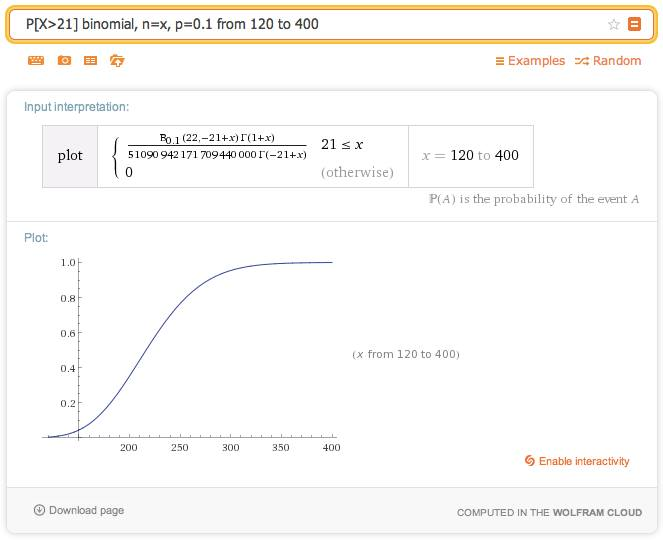
\includegraphics[scale=0.75]{graph}

As the number of users increases, it becomes more and more of a sure bet that more of them will be using the line simultaneously. This probability never approaches 1, since there is always a small chance, no matter how unlikely, that no users will be using the line.

\newpage
\stepcounter{set}
\problem

The queuing delay $d$ for packet $i$ is $d_{i} = i \cdot d_{trans}$. The average queuing delay is thus:

let $d_{trans} = L/R$

\begin{align*}
d_{avg} &= 
\sum_{i=0}^{n-1} i \frac{d_{trans}}{n} \\
&= \frac{d_{trans}}{n} \sum_{i=0}^{n-1} i \\
&= \frac{d_{trans}}{n} \frac{n(n-1)}{2} \\
&= d_{trans} \frac{(n-1)}{2} \\
\end{align*}


\end{document}